\documentclass[runningheads,a4paper]{llncs}
\usepackage{amsmath,amssymb,amsfonts,mathrsfs,stmaryrd}
\usepackage{bussproofs}
\setcounter{tocdepth}{3}
\usepackage{graphicx}
\usepackage{multirow}
\usepackage{booktabs}
\usepackage{algorithm2e}
\usepackage{wrapfig}
\usepackage{url, listings, color}
%\usepackage{hyperref}

%two column float page must be 90% full
\renewcommand\dblfloatpagefraction{.99}
%two column top float can cover up to 80% of page
\renewcommand\dbltopfraction{.99}
%float page must be 90% full
\renewcommand\floatpagefraction{.99}
%top float can cover up to 80% of page
\renewcommand\topfraction{.99}
%bottom float can cover up to 80% of page
\renewcommand\bottomfraction{.99}
%at least 10% of a normal page must contain text
\renewcommand\textfraction{.01}

\newcommand{\code}[1] {{\footnotesize\sffamily #1}}
\newcommand{\transml}[1]{{\textit{trans}ML\ }}

\titlerunning{Engineering BX}
\authorrunning{Richard F. Paige}

\begin{document}

\title{Engineering Bidirectional Transformations}

\author{
Richard F. Paige, richard.paige@york.ac.uk}
%
\institute{
University of York, United Kingdom
}

\maketitle

\begin{abstract}
Bidirectional transformations, like software, or model and program transformations in general, need to be carefully engineered in order to provide guarantees about their correctness, completeness, acceptability and usability. This paper summarises a collection of lectures pertaining to engineering bidirectional transformations using Model-Driven Engineering techniques and technologies. It focuses on stages of a typical engineering lifecycle, starting with requirements and progressing to implementation and verification. It summarises Model-Driven Engineering approaches to capturing requirements, architectures and designs for bidirectional transformations, and suggests an approach for verification as well. 
\end{abstract}

\section{Introduction}
\label{section:introduction}

This paper describes a set of lectures on a collection of techniques and tools that can be used for engineering bidirectional transformations (BX). The motivation for these lectures is our view that transformations in general -- and BX in the specific -- are like other software systems: they are designed to be executed on a machine, are complicated (and in some cases even complex), and are difficult to build correctly. As such, like software, transformations should be engineered by following a rigorous process. The advantages of doing so are the same as for software, including:
\begin{itemize}
\item \textit{Repeatability:} by following a process, we potentially make it easier for others to repeat our work, or to reduce the amount of effort required to build a similar system in the future.
\item \textit{Review and Scale:} by decomposing a large engineering problem into stages, we potentially make it easier to audit and validate the results of each stage, and to solve larger problems than we would be able to if we treated the problem monolithically.
\item \textit{Automation:} by following a process we have greater opportunities to automate parts of it, e.g., generation of code or documents. 
\item \textit{Training:} by following and documenting a rigorous engineering process we may make it easier to train others.
\end{itemize}
BX are special kinds of transformations with, in our opinion, complicated execution semantics. As such, BX may especially benefit from following a repeatable, reviewable, scalable, automated process with training/guidance, for their development.

\subsection{BX as software}
The assumption that we are making in the preceding is that BX are software systems. A software system is an executable artefact: given a specification of software (e.g., in a programming language or suitable modelling language), its expected outputs can be produced by executing the specification on a suitable machine (e.g., a server, a virtual machine, a simulator). A BX is an executable artefact: assuming that the BX is expressed in a suitable programming language or modelling language (and we review some of the key state of the art in Section~\ref{section:state-of-the-art}) then its expected outputs can be produced by executing the BX on a suitable machine. 

Like software, BX must satisfy functional and non-functional requirements, can (and probably should) be designed, and can exhibit unacceptable behaviour -- that is, BX can contain bugs or faults, which may lead to failures. As we will see, depending on the technologies used to represent and specify BX, different types of failures may arise (e.g., inconsistencies) and different techniques may be used to verify the BX to help ensure that faults are caught during engineering. As we become increasingly ambitious in our attempts to solve complex problems using BX, our need for rigorous engineering techniques for BX construction will only increase.

\subsection{Scope}
There are numerous techniques and approaches that can be used to build and engineer BX; in Section~\ref{section:state-of-the-art} we will consider some of these. However, the focus of this paper will be on Model-Driven Engineering (MDE) techniques, because of our experience with them. Many of the techniques that we present in later sections can be used both with and without MDE tools, and if there are particular aspects that depend specifically on MDE, we will point these out where such a dependence isn't clear.

\subsection{Background}
Before we commence with the technical content of this paper, we provide some basic definitions and terminology, in order that the paper remain reasonably self-contained.

As mentioned, we are focusing on Model-Driven Engineering techniques for engineering BX. The key concepts of MDE are as follows.

\begin{itemize}
\item MDE involves the semi-automated construction and manipulation of \textit{models}, which are structured, machine-implemented specifications of phenomena of interest. Models are meant to be processable by automated tools, and capture static and dynamic characteristics of systems. 

\item Models in MDE are \textit{structured}; this structure can be defined in a number of ways, including via \textit{metamodels}, which are specifications of abstract syntax (you can think of a metamodel as a the definition of the abstract syntax of a language). 

A model is said to \textit{conform} to a metamodel. Related approaches to defining the structure of models include schemas (e.g., XML), type rules and constraints. Many of these approaches define structure using graphs or graph-like concepts. As such, models themselves are typically graphs. This is a key distinction between MDE (and so-called \textit{modelware} approaches to engineering), and grammar-based (or \textit{grammarware}) approaches.

\item Models are typically specified alongside a set of \textit{constraints} that capture well-formedness rules that cannot normally be specified with a metamodel. For example, a metamodel might be used to express that a model may include containers, and that containers may be nested (e.g., packages in Java or UML). But a metamodel -- which captures abstract syntax -- will not normally express that containers have unique names. This can be expressed by a separate constraint, which is normally packaged up with the metamodel or models. If a model conforms to a metamodel, it must also normally be checked against any constraints, in order to establish that it is well formed.

\item Standard technologies exist for capturing models, metamodels and constraints in the MDE world. The de facto standard technology used for metamodelling is Ecore (a part of the Eclipse Modelling Framework (EMF)). For constraints, engineers typically use the Object Constraint Language (OCL), which also has an official Eclipse implementation. There are other languages and technologies available as well (e.g., typed graphs, MetaDepth, XMI) for metamodelling and for expressing constraints.

\item Models by themselves typically encapsulate business value, but are also meant to be processed by automated tools. These tools implement a variety of operations applicable to models, including the aforementioned transformations, but also comparisons, merging, migration, matching and others.
\end{itemize}

Transformations are a key operation in MDE, and have been the subject of widespread study (e.g., see the proceedings of the long-running conference on model transformation, such as \cite{icmt2016} ). Numerous classifications and surveys have been published on transformations in general, and BX in the specific. Four common categories of transformations in MDE are:
\begin{itemize}
\item \textit{Unidirectional transformations}, from a source model to a target model. Such transformations are usually implemented in terms of metamodels, and are typically used when the source and target metamodel are linguistically similar, e.g., between different dialects of UML, or from an object-oriented model to a relational database model. Unidirectional transformations typically are written in one of three styles: purely declarative, operational, and hybrid (i.e., a mixture of operational and declaration parts). In our experience, many complicated transformations are very difficult to express in a purely declarative style, and as such hybrid unidirectional transformation languages (such as ATL \cite{JouaultABK08} and ETL \cite{Kolovos2008}) tend to see the most use in practice.

\item \textit{Update-in-place transformations}, which specify modifications made to one and only one model. Update-in-place transformations can be specified using languages suitable for unidirectional transformations, or specialist languages such as EWL \cite{KolovosPPR07}.

\item \textit{Model-to-text} (sometimes called model-to-grammar) transformations, where the source/input to the transformation is a model, but the output is no longer a model, e.g., free-form text or text conforming to a grammar. Model-to-text transformations are used in order to step outside of the modelware technical space and move to the grammarware technical space. An example scenario for use of model-to-text transformation is code generation.

\item Bidirectional transformations, which is the subject of the next section.
\end{itemize}
Transformations (and other operations on models) have side-effects. This includes purely declarative transformations. The side-effect in question is the production of \textit{traceability} information, i.e., so-called \textit{trace-links}, which relate source and target model elements. Trace-links can be generated automatically by transformation tools (such as Epsilon or ATL) and they can be stored for later audit and analysis. Trace-links are important in the context of transformations and BX as they provide (a) the basis for verification and validation of transformations; and (b) the connection to the theory behind BX, specifically delta lenses (in particular, delta lenses are a sound theory for trace models, encoded in an algebraic form \cite{DiskinXC10}).

\subsection{Structure of paper}
The paper starts with a brief review of the state-of-the-art in engineering BX with MDE, focusing firstly on BX scenarios of use in MDE, followed by an overview of MDE languages, tools and techniques for supporting BX. The remainder of the paper considers different aspects of a BX engineering lifecycle, starting with an overview of techniques for requirements engineering for BX, focusing on requirements specification and requirements analysis. We then move to an overview of techniques for architecture and design of BX, including a small selection of relevant design patterns. Finally, we briefly consider one approach for verification of BX, which applies to a specific approach to BX implementation and design. The paper concludes with a discussion on future challenges and perspectives on engineering of BX.



\section{State of the Art}
\label{section:state-of-the-art}

This section addresses some of the important state of the art in MDE approaches to BX, focusing on three specific elements: important BX \textit{scenarios} that have been identified in the literature; important \textit{languages} that have been influential in research in BX -- in this case, we focus on QVT; and important \textit{tools} that implement aspects of BX and that are based on MDE technology. We do not consider non-MDE approaches to BX in this brief review, and we also exclude TGG approaches because these are covered in detail by other lectures in this volume\footnote{Comment: replace this by a reference to Tony's paper once the final citation format for the volume have been specified.}.

\subsection{BX Scenarios}
A number of recurring scenarios of use for BX have appeared in the MDE literature. Many of the MDE tools and languages that we discuss in the sequel have been designed to address these scenarios.

\begin{enumerate}
\item \textit{Round-trip engineering}, i.e., generating code from models, modifying the code by hand, and then regenerating the models to reflect changes made in the code. A BX approach would, conceptually, aim to apply the principle of least change and minimise the number of modifications necessary to the original model, instead of regenerating the entire model after each change. Research in MDE related to incremental transformation is also addressing this scenario.

\item \textit{Collaborative modelling}, wherein multiple stakeholders are editing the same model simultaneously. In practice, what often happens is that each stakeholder has a local copy (or view) of the source model, and their changes are reflected back on the master/source copy at specified points of time.

\item \textit{Synchronisation,} e.g., synchronising documents and code, like assurance cases and source code. This is related to round-trip engineering but synchronisation can involve model management operations other than transformations.

\item \textit{Reflection,} for example, reflecting the results of some kind of analysis on a source model. A concrete instance of this was investigated in the MADES project\footnote{\url{http://www.mades-project.org/}} where a UML MARTE model was transformed into a variety of formal models (UPPAAL, TRIO) to support analysis, and some of the results of the analysis were reflected in the MARTE models. This is an interesting example of a BX as the backwards transformation is generating a view of the target model which needs to be synchronised with the source model.
\end{enumerate}

\subsection{Standard MDE languages for BX: QVT}
While there are tools and approaches, based on MDE technology (like Eclipse EMF) for supporting BX, most of these approaches are strongly influenced by a significant standardised language for transformation: the OMG's Query, View and Transformations (QVT) standard \cite{QVT-specification}. QVT is a family of languages that were first envisaged in 2002 upon issue of an OMG request for proposals to support aspects of the OMG's Model-Driven Architecture standard. A number of replies were received, and the first version was submitted and approved in 2005. The most recent version, QVT 1.3, was released in June 2016. 

QVT, as mentioned, is a family of languages. These languages are meant to support transformation and querying of MOF models; transformations and queries  can be used in turn to generate views. The basic architecture of QVT is illustrated in Figure~\ref{fig:qvt}. The QVT architecture builds on other OMG languages, particularly MOF but also the Object Constraint Language (OCL), from which QVT acquires its expression and collection manipulation facilities.

\begin{figure}[htbp]
\centering{\scalebox{0.5}{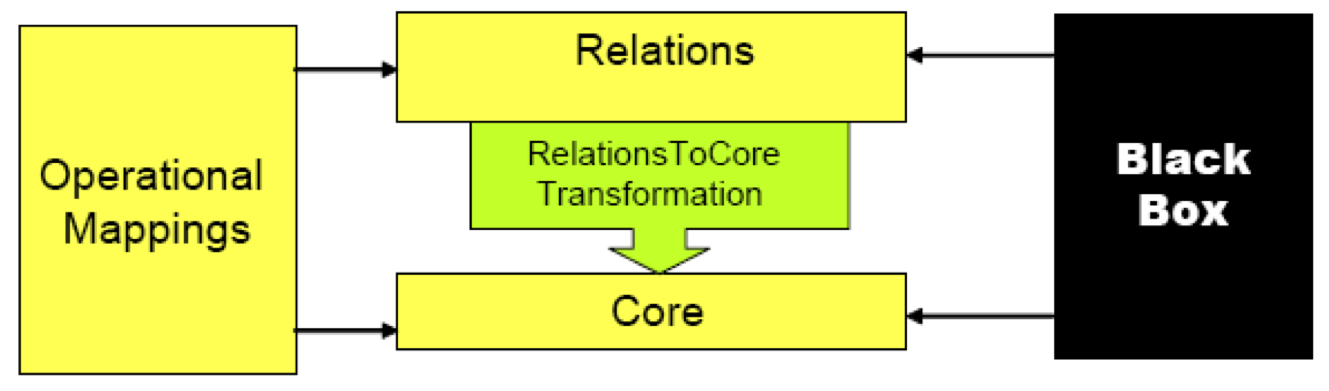
\includegraphics{qvt-architecture.png}}}
\caption{QVT architecture \cite{QVT-specification}}
\label{fig:qvt}
\end{figure}

The Relations language provides mechanisms for the declarative specification of the relationships between MOF models. It supports in turn complex object pattern matching, and implicitly creates trace classes and their instances to record what occurred during the execution of a transformation. Assertions can also be made; for instance, relations can assert that other relations also hold between particular model elements matched by their patterns. As illustrated in the figure, the intention is that Relations specifications can be translated in to the QVT Core language, along with a set of trace models, which in total provide a formal semantics for QVT Relations.

QVT Core, by contrast, is a small yet expressive language that only supports pattern matching over a flat set of variables by evaluating conditions
over those variables against a set of models. It is intended to be semantically equivalent to QVT Relations, but equivalent QVT Relations programs are liable to be more concise than the QVT Core programs.

The Operational Mappings (sometimes called QVT Operations, or QVT-o) is an operational model transformation language that extends Relations with imperative constructs. Of all the QVT languages, it is QVT-o that has received the most use and attention.

\begin{figure}[htbp]
\centering{\scalebox{0.6}{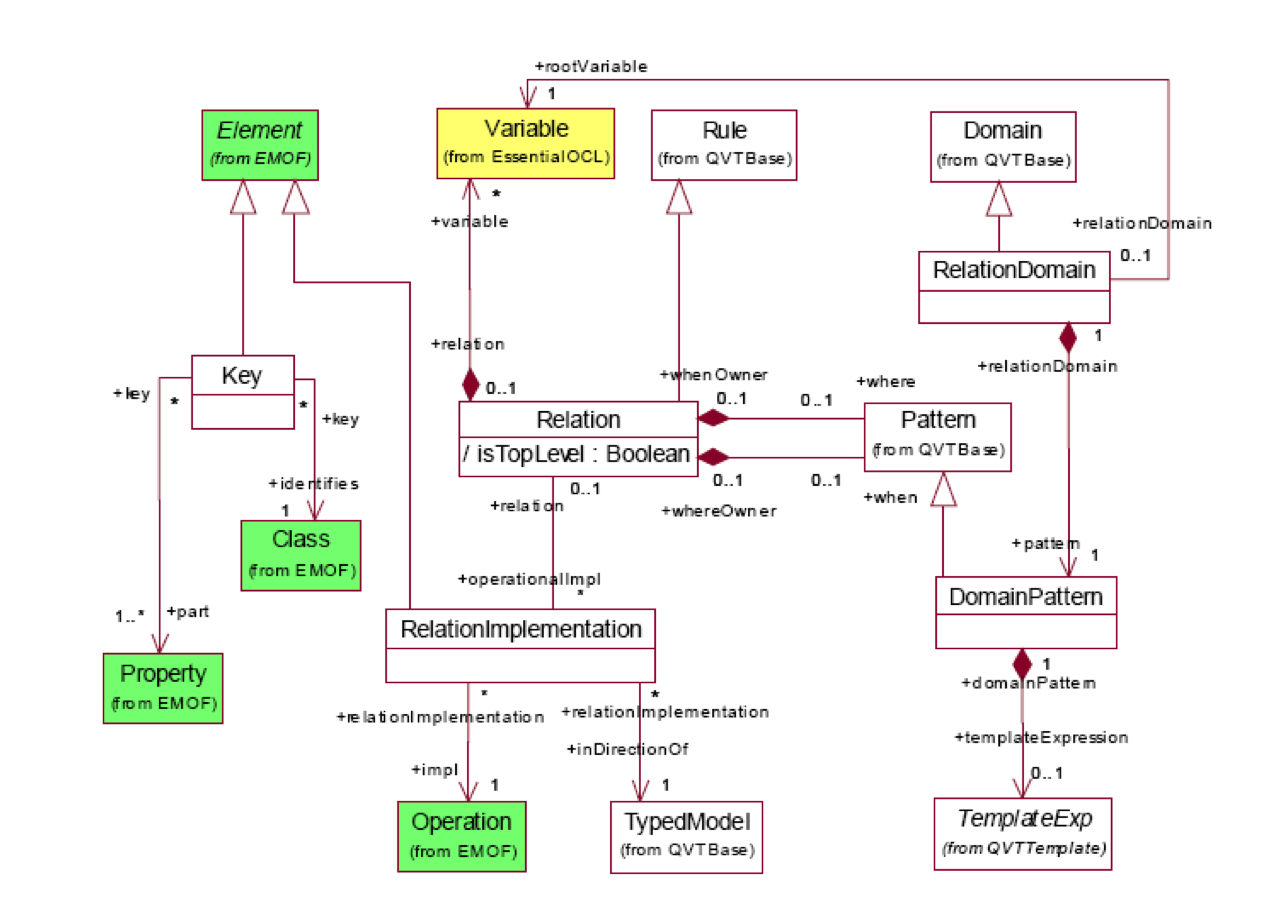
\includegraphics{qvt-relations-metamodel.png}}}
\caption{QVT Relations abstract syntax}
\label{fig:qvt-as}
\end{figure}

The abstract syntax of the Relations language is illustrated in Figure~\ref{fig:qvt-as}. The abstract syntax can be interpreted as follows: a QVT Relations program contains a set of rules which are relations. Relations are made up of patterns, and are applied to a set of typed model parameters. In particular, these relations can be interpreted in forward and backwards directions -- that is, Relations is a BX language by design.

An example of the concrete syntax of Relations is shown in Listing~\ref{listing:qvt-relations}. This example gives a relation that is part of the classic object-relational mapping, in this case used to map persistent classes in an object oriented program to a table. The example includes three parts: a domain (a set of patterns which defines the variables and constraints that model elements bound to those variables must satisfy -- i.e., the bindings for the relation); the \textit{when} clause (the conditions under which the relation must hold); and the \textit{where} clause (the condition that must be satisfied by all model elements participating in the relation). The interpretation of when-clauses in the Eclipse QVT implementation is that these are preconditions, and where-clause are postconditions. Both of these clauses may contain arbitrary OCL expressions.

\begin{lstlisting}[float,floatplacement=H,basicstyle=\ttfamily,caption=An example of QVT Relations, label=listing:qvt-relations]
relation ClassToTable /* map persistent class to table */
{
  domain uml c:Class {
      namespace = p:Package {},
      kind = 'Persistent',
      name = cn
  }
  domain rdbms t: Table {
      schema = s:Schema {},
      name = cn,
      column = cl:Column {
        name = cn + '_tid',
        type = 'NUMBER'},
        primaryKey = k:PrimaryKey {
          name = cn + '_pk',
          column = cl }
   }
   when { 
     PackageToSchema(p,s);
   }
   where {
      AttributeToColumn(c,t);
    }
}
\end{lstlisting}
In this particular example, the domain clauses establish which model elements in a UML and a RDBMS model are of interest (they satisfy the predicate part of the domain clauses), and the when and where clauses are defined elsewhere by other relations.

The BX capabilities of QVT can also be illustrated by an example from QVT Core. Figure~\ref{fig:qvt-core} illustrates an example of a single mapping rule in QVT Core. This is a \textit{checking} example, which is used to check that particular patterns are satisfied by models. Once again, this is an example involving relations between a UML class model and a database model. The top part of the diagram (labelled Class to Table) defines the \textit{c2t} relation, which relates a class to a table. The bottom pattern is evaluated using variable values of a valid binding (a valid pair of class and table) from the top pattern. In effect, the top part of the mapping rule defines a guard which restricts the scope of the bottom part of the rule.

\begin{figure}[htbp]
\centering{\scalebox{0.5}{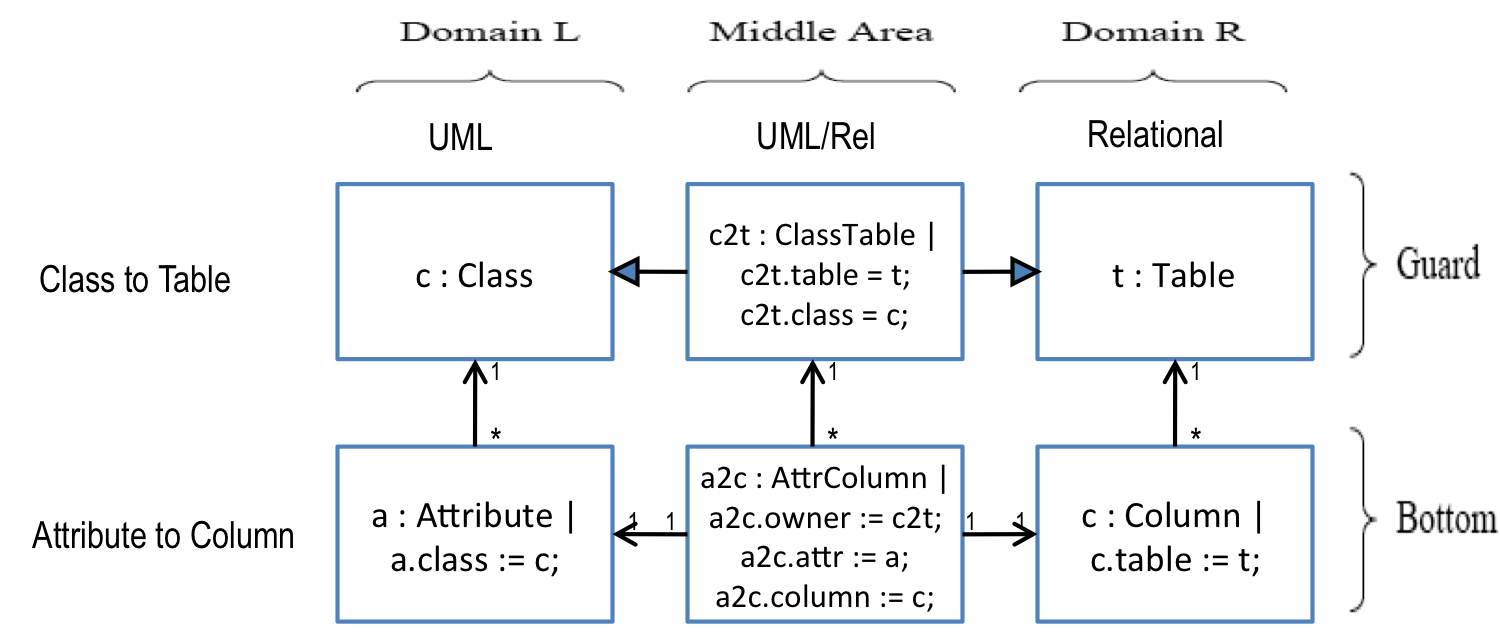
\includegraphics{mapping-rule.png}}}
\caption{QVT Core: mapping rule example}
\label{fig:qvt-core}
\end{figure}

The mapping rule is directionless; it can be executed either way, i.e., checking a database table against a UML class, or checking a UML class against a database table.

The QVT standard is currently being further developed, both through the OMG standardisation efforts, but also through work on Eclipse QVT, an implementation of the different QVT languages. We briefly discuss the status of Eclipse QVT, and other MDE tools for BX, in the next subsection.

\subsection{Tools}
In this section we briefly outline some of the key tools, based on MDE technologies and principles, that either support or claim to support BX. As mentioned earlier, we exclude approaches based on triple graph grammars as these are covered elsewhere.

\subsubsection{Medini}
Medini\footnote{\url{http://projects.ikv.de/qvt/wiki}} claims to be a reasonably complete implementation of QVT Relations, but is currently unsupported. It is an EMF based transformation engine but also has a non-commercial licensed editor and debugger. While it uses the the QVT Relations syntax, it intentionally departs from the semantics of the OMG standard (e.g., how it supports deletion of elements, that it does not provide a checkonly mode). As such, we prefer not to label Medini as an implementation of QVT, but as a tool that is inspired by QVT.

\subsubsection{ModelMorf}
ModelMorf is a proprietary tool from Tata Consulting Services\footnote{Archived copy available at \url{https://web.archive.org/web/20120323171429/http://www.tcs-trddc.com/trddc_website/ModelMorf/ModelMorf.htm}}. It also claims to faithfully implement the QVT Relations standard, but research by Stevens \cite{Stevens13} shows that it does not fully implement the semantics specified in the standard. By some measures, it is more faithful than Medini, but it is still not a full implementation of QVT.

\subsubsection{jQVT}
jQVT\footnote{\url{https://sourceforge.net/projects/jqvt/}} is a QVT-like engine that is defined on top of the Java type system instead of using EMF. In turn, it uses Xbase (a partial programming language written in Xtext which compiles to Java and includes powerful features such as closures) instead of OCL for expressions. In essence, jQVT is a Java embedding of QVT; the jQVT engine generates native Java code from jQVT scripts. Of note is that it does provide support for bidirectional transformations. As of early 2016 jQVT was still being maintained.

\subsubsection{Echo}
Echo\footnote{\url{http://haslab.github.io/echo/}} is an open-source EMF-based tool for model repair and transformation that exploits the Alloy model finder to determine models that satisfy relations. It provides an implementation of the QVT Relations syntax, but the semantics intentionally departs from the OMG specification. Echo is also bidirectional.

\subsubsection{JTL}
The Janus Transformation Language (JTL)\footnote{\url{http://jtl.di.univaq.it/}} is a by-design bidirectional language with a QVT-like syntax, which propagates changes made in one model to the other. If a change made to one model makes the second model inconsistent, an approximation (``closest match'') is calculated using answer set programming. As such, there can be several solutions to a transformation problem and the results provided by JTL may need to be constrained further.

\subsubsection{Eclipse QVT}
Substantial engineering effort is being put into the development of Eclipse QVT, a project that
aims to support the full OMG QVT specification (though with Ecore instead of MOF models). Currently, QVT Operations is well supported and active as part of the Eclipse M2M project. QVT Relations (in Eclipse terms, QVT Declarative) and QVT Core are work-in-progress. As work on these projects is ongoing and their status is changing regularly, we refer the reader to the Eclipse MMT project website\footnote{\url{https://projects.eclipse.org/projects/modeling.mmt}} for the latest information. As of this writing, the intention with Eclipse QVT is that the Oxygen release in June 2017 will provide full support for QVT Relations.

\subsubsection{Bidirectionalisation}
There have been several approaches to so-called \textit{bidirectionalisation} of transformations. In these approaches, a forward transformation (from source to target) is written and the backward transformation is calculated or computed automatically. Examples of this approach include that of Hoisl \cite{HoislHH14a}. The GRoundTram approach of Sasano \cite{SasanoHHIKN11} is another example.

\vspace{4mm}

For further details, and a more in-depth classification of MDE approaches to BX, the interested reader is referred to Hidaka et al's excellent survey of BX \cite{HidakaTCH16}.




\section{Requirements Engineering for BX}
\label{section:requirements}

In this section we will consider techniques and tools for requirements engineering for BX. We will motivate the benefits of considering requirements for BX in general, before discussing some of the general questions to be addressed when building a BX. These questions will help us motivate a discussion on the general properties of BX (which may be the source of constraints on requirements for a BX), as well as examples of functional and non-functional requirements for BX. This is followed by a broad overview of requirements engineering processes for BX, which leads in to a discussion on MDE languages suitable for requirements engineering for BX.

\subsection{Motivation}
Requirements engineering is the process of identifying, documenting and maintaining requirements in systems engineering. The typical tasks involved in requirements engineering are:
\begin{itemize}
\item \textit{identification:} where new requirements to address a problem are clarified
\item \textit{analysis:} where the requirements are assessed to ensure they accurately capture what is needed for the system under consideration, and conflicts between stakeholders are resolved
\item \textit{specification:} where the requirements are documented in a precise (but not necessarily formal) way
\item \textit{validation:} where the requirements are checked to ensure they are consistent and address stakeholder needs
\item \textit{maintenance:} where the requirements are considered for update as the system under consideration is constructed, deployed and changed.
\end{itemize}
BX are software systems and as such will benefit from a clear understanding of requirements; for large or complicated BX, there may be benefits to following a rigorous requirements engineering process as well. In particular, an understanding of requirements for BX can help in mapping BX problems to tools that are suitable for implementation (and vice versa). An understanding of requirements for BX can also help in contrasting different potential solutions in terms of their tradeoffs in how they satisfy requirements.  

\subsection{Questions and Properties for BX}
A typical first phase of requirements engineering is \textit{identification}, where engineers attempt to determine what requirements a software system should exhibit. This in turn may help determine properties or constraints that the ultimate system will satisfy. There are numerous ways in which requirements can be identified, e.g., via stakeholder interview, by reviewing existing similar systems, by following questionnaires or checklists, or by using testing techniques to derive requirements. Based on \cite{TehraniZL16} we suggest some general questions that could be addressed when constructing a BX, the answers to which could help derive requirements.

\begin{enumerate}
\item What needs to be transformed into what?
\item What mechanisms can be used for building the BX? (i.e., theory, tools, techniques)
\item What are the application domains for the BX?
\item What are the specific characteristics of the BX (e.g, what patterns are appropriate to use)?
\item What are the quality requirements (e.g., performance) for the BX?
\item What are the success criteria for the BX?
\end{enumerate}
Questions 3, 4 and 6 are possibly the most opaque. Question 3 is designed to help identify constraints on the scope of use for the BX, e.g., will the BX be used in developing hard real-time systems, or interactive systems? Question 4 is designed to help identify functional requirements, e.g., should the BX be parameterised, should it be interactive? This in turn may help identify suitable patterns that can be used in specifying or designing the BX. Question 6 is the ``stopping condition'': how will we know if we have successfully solved the BX problem?

BX exhibit various properties (such as least-change, or determinism). When considering requirements for a BX, there are general properties that may be of interest, particularly in determining constraints that the ultimate BX must satisfy. Some examples are:
\begin{itemize}
\item Size: is the BX small (e.g., a single reversible refactoring) or large (e.g., a reversible code generator)? 
\item Level of automation: is the BX meant to be fully automated, or involve a human-in-the-loop?
\item Visualisation: how is the BX, its results, and its input presented to users?
\item Level of industry application: to what extent is the BX to be deployed in an industrial context?
\item Maturity level: should the BX be implemented in a tool? Should the BX be a theoretical construct?
\end{itemize}
Understanding the relative importance of these properties will be helpful in deciding on what theory or tool to choose for defining a BX.

\subsection{Functional and Non-functional Requirements}
In the classical requirements engineering literature, functional requirements specify what a system must, could or should provide. Non-functional (or behavioural) requirements specify criteria against which we can judge the quality of a system. In a requirements document, functional and non-functional requirements are typically presented separately, with suitable tests given that can be used to assess the coverage and completeness of fulfilment of requirements.

There has been little published research on examples of requirements for transformations in general, let alone BX, but based on \cite{TehraniZL16,NalchigarSC13} we can propose some examples for BX. We start with functional requirements. For simplicity of presentation, we assume that a BX under development is defined between two models (a source and a target).

\begin{itemize}
\item \textit{Correctness:} when the BX is run in the forward direction, the target model must be well formed (defined in terms of conformance to the target metamodel and any corresponding constraints). Similarly, when the BX is run in the reverse direction, the source model must be well formed.

\item \textit{Inconsistency tolerance:} the BX should be able to support incomplete or inconsistent models, e.g., temporarily inconsistent models. This reflects the practical situation wherein a BX \textit{gradually} re-establishes consistency over a sequence of steps.

\item \textit{Modularity:} it should be possible to compose BX into new transformations.

\item \textit{Traceability:} a BX should support the generation of trace-links (sometimes called a correspondence model) between source and target models, as well as between the steps of a transformation chain.

\item \textit{Change propagation:} a BX should provide support for propagating changes from one model to the other model. 

\item \textit{Incrementality:} a BX should make it possible to update a model based only on the changes made to the other model (that is, the parts of the model that do not change are not used to make changes to the other model). 

\item \textit{Uniqueness:} a BX could support the ability to generate a unique solution to the problem of ensuring consistency between two models.

\item \textit{Termination:} it should be possible to support the definition of terminating BX transformation executions.

\item \textit{Style:} a BX should be expressible in a particular style, i.e., declarative, operational or hybrid. 
\end{itemize}
Note the wording of these requirements; we have used the words \textit{must}, \textit{should} and \textit{could} to indicate the degree of importance or criticality of each type of requirement. As this suggests -- and as is reinforced by \cite{HidakaTCH16} there is substantial variability in what BX provide (and also how they are implemented).

Non-functional requirements, recall, specify criteria against which we can judge the quality of a BX. As is the case for functional requirements for BX, there is limited research on non-functional requirements. Some examples have been proposed in \cite{NalchigarSC13}, and we list a selection here.

\begin{itemize}
\item Extensibility: the extent to which the BX can be extended to support new functional requirements  or a change in scope.

\item Usability: is the BX judged to be usable by stakeholders?

\item Robustness: can the BX manage invalid models (i.e., that do not conform to the metamodels involved in the BX), or deal with errors in models?

\item Interoperability: can the BX be combined and used together with non-BX tools (e.g., other MDE tools and operations, such as model comparisons or mergings)?
\end{itemize}

Clearly, more research on requirements for BX is needed. As our experience with building BX grows, and our understanding of what constitutes a useful BX scenario increases, our ability to elaborate sensible functional and non-functional requirements for BX will improve.

\subsection{Requirements Engineering Processes for BX}
In this section we briefly outline typical stages of a requirements engineering process for BX and highlight the key artefacts and stakeholders that will be involved. We discuss elicitation in some detail, and evaluation briefly. This leads in to the next section where we give an overview of some of the key specification techniques that can be used within a requirements engineering process for BX.

The requirements engineering literature, e.g., \cite{ieee-29148-2011}, identifies the following generic phases in requirements engineering:
\begin{itemize}
\item \textit{Domain analysis and elicitation:} Identify who are your stakeholders. From these stakeholders, gather information on the system domain and system requirements.

\item \textit{Evaluation and negotiation:} Identify imprecision, conflicts, omissions and redundancies in the informal requirements identified in the previous phase.  Resolve these (if possible and appropriate) via negotiation and consultation.

\item \textit{Specification:} Document the formal requirements in a specification (we will consider this for BX in more detail later). The specification is often the basis for a contract between developers and customers.

\item \textit{Validation and Verification:} Check the specification for consistency, completeness and acceptability to stakeholders.
\end{itemize}

This is generic, applicable to any kind of software or systems engineering. What might a requirements engineering process for BX look like? Tehrani et al \cite{TehraniZL16} propose a process for transformations, which is depicted in Figure~\ref{fig:re-process}.

\begin{figure}[htbp]
\centering{\scalebox{0.5}{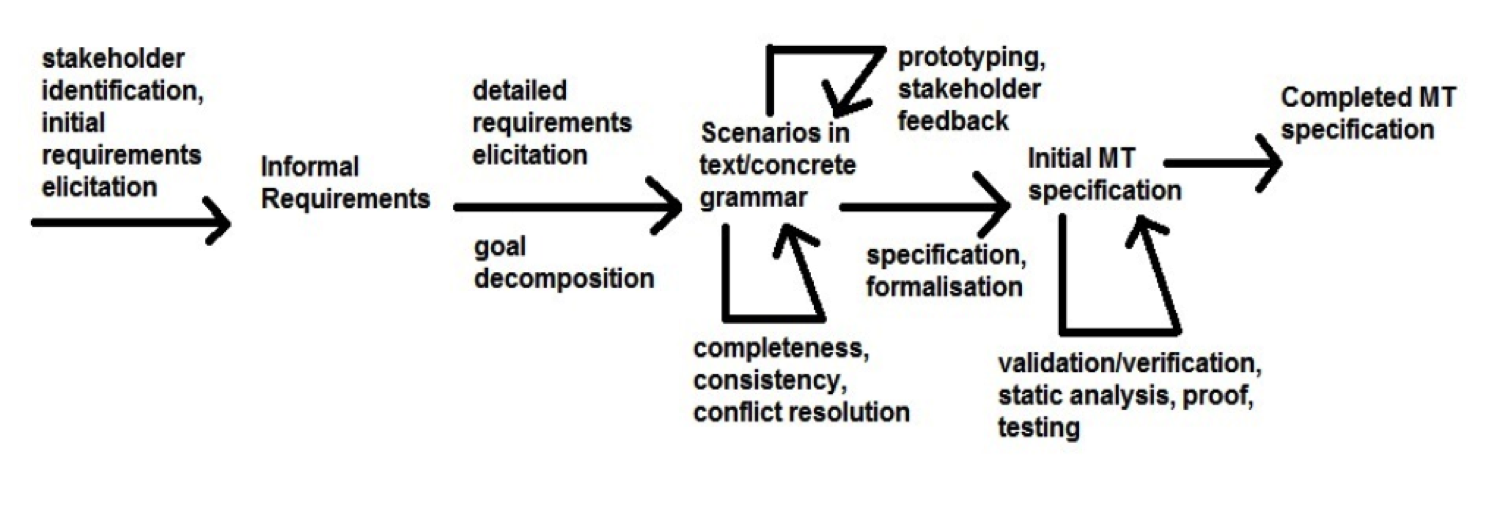
\includegraphics{re-process-bx.png}}}
\caption{A requirements engineering process from \cite{TehraniZL16}}
\label{fig:re-process}
\end{figure}
(It is worth emphasising that the process shown in Figure~\ref{fig:re-process} is for transformations in general, not specifically for BX.) There are some points to note about the above process.

\begin{itemize}
\item The process is generic for the most part, and resembles the steps that are typically carried out for software systems.

\item An interesting aspect is the use of scenarios as a concrete mechanism for driving the development of a requirements specification. In the context of BX this suggests that identifying and capturing more (and more detailed) BX scenarios will be very helpful in improving our understanding of BX requirements engineering.

\item The process distinguishes between local and global requirements, as is often done in systems engineering. A local requirement may pertain to a particular transformation component (e.g., that correspondences are defined between elements of particular types), whereas a global requirement may apply to an entire transformation (e.g., a performance requirement, that a measure of complexity is reduced by running a BX, or a safety requirement).
\end{itemize}

\subsection{Elicitation}
\textit{Elicitation} is an important first step in any requirements engineering process. What techniques might be applicable for BX? Many of the traditional elicitation techniques appear to be directly applicable to BX problems with little change, as argued by Tehrani et al \cite{TehraniZL16}. For example, a classic elicitation technique is observation (an ethnographic method): observing an existing -- possibly manual -- BX technique or process could provide sensible requirements for an automated process. Consider a scenario wherein a BX is to be defined between an Excel spreadsheet and a SysML requirements diagram\footnote{This is a sanitised version of a real problem encountered by the author.} A manual BX process between the two might involve (a) making changes to cells in an Excel column; (b) switching to a SysML editor; and (c) modifying attributes in a SysML class model. This might indicate to a requirements engineer a sequence of steps that is needed to implement in an automated BX.

Another technique that can be used for elicitation is the \textit{unstructured interview}, where open-ended questions are asked about the problem domain or the current (BX) process. This can be useful for identifying transformation goals, e.g., ``ensure that the source and target models are inconsistent for no more than 10ms''. In carrying out an unstructured interview regarding a transformation, Tehrani \cite{TehraniZL16} suggests some generic open-ended questions that may be useful to consider; we have extended their questions with some of our own, based on our experience in the MONDO project\footnote{http://www.mondo-project.org/}.
\begin{itemize}
\item Is there a size range for the source and target models? This may suggest to the engineer the type of infrastructure that may be useful for the project (e.g., EMF to represent models).

\item Does the encoding for the BX matter? For example, for very large scale models it may be necessary to consider binary formats.

\item Are there any assumptions that are made about the source or target models? For example, are they always available? Are they read-only? Write-only? Are there confidentiality restrictions?
\end{itemize}
Along with unstructured interviews there are \textit{structured} interviews, which involve asking pre-loaded questions about the domain and the BX, perhaps based around a checklist linked to a requirements pattern catalogue. For example, a checklist of questions may be divided into parts, one focusing on questions related to global functional requirements (e.g., is hippocraticness important, is semantics preservation important?) and another related to local non-functional requirements (e.g., should this rule satisfy a specific time bound?)

A final elicitation technique that we mention is \textit{scenario-based analysis}, where scenarios are used to capture different requirements transformation processing cases. The benefit of using scenarios is that they are concrete: scenarios are usually presented in a concrete scenario language, often supplemented with sketches of sample models. For example, for BX we might specify a scenario for introducing or removing a pattern to change an object-oriented design. The forward transformation scenario could include a concrete example of introducing the pattern into an existing design.

\subsection{Evaluation}
Once we have elicited requirements for BX through any of the techniques described previously, we have a set of informal statements of what the BX must or should provide. These statements may be inconsistent, and ideally we should be identify this before we formalise the BX requirements in a specification. There is little to no published research on evaluation techniques for BX requirements. We may find some inspiration in the general requirements engineering literature. For example, one approach used for requirements evaluation is prototyping, i.e., engineers build a prototype (paper, mock-up, simulation) of a solution in order to help identify or reconcile inconsistencies. It is unclear whether the expense of building a BX prototype is greater than building a BX in the first place (because, for example, a BX prototype would need to be constructed using standard BX tools). Another approach that is sometimes used is goal-oriented analysis, but it is as of yet unclear  how goal-oriented techniques apply to the definition of BX. There are significant open questions relating to how we evaluate requirements for BX.

\subsection{MDE Languages for Requirements Engineering for BX}
In this section we move from a mostly abstract discussion on requirements engineering for BX and focus on the more concrete topic of languages that can be used to support requirements engineering for BX. There has been some work in this area -- i.e., on different MDE languages and tools for specifying transformation requirements -- though there is still very limited experience of specifying requirements for BX in the specific. Here, we will focus on presenting details of one approach -- \transml\ -- which is a family of languages that can be used for engineering model transformations. \transml\ can, as we will show, be used to specify different aspects of the requirements for a BX. We will also use \transml\ in the next section to specify different facets of the architecture and design of a BX. For an alternative approach to specifying requirements for transformations, based on mind-maps, the interested is referred to the DSL-Maps approach \cite{PescadorL16}.

\transml\ \cite{GuerraLKPS13} by way of introduction, is a family of MDE languages to support the lifecycle of transformation development, from requirements through to implementation. It is technology agnostic, and can be used with any transformation implementation language (there is published experience of using \transml\ with QVT, EOL, ETL and ATL). The overall architecture of \transml\ -- that is, the set of languages and their inter-relationships -- is depicted in Figure~\ref{fig:transML}. The parts of \transml\ relevant to this section are the Requirements language (at the top) and the languages to support Analysis (Simple Scenarios and Formal Specification).

\begin{figure}[htbp]
\centering{\scalebox{0.6}{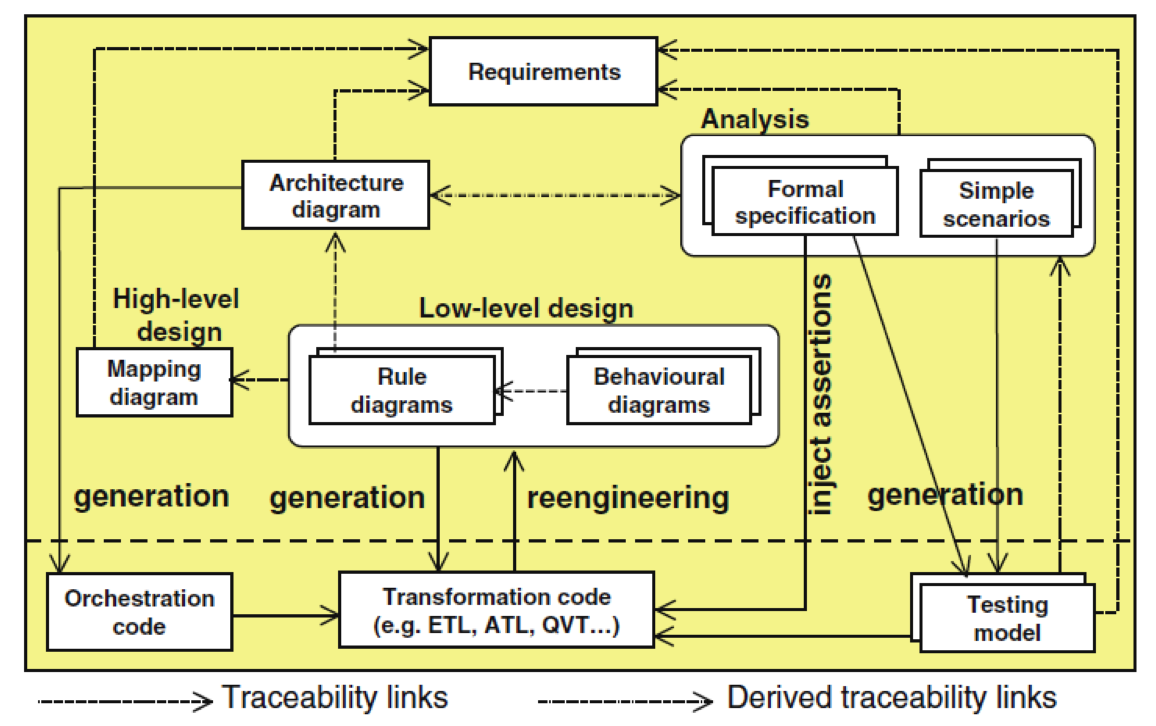
\includegraphics{transml.png}}}
\caption{\transml\ architecture; boxes represent languages (or sets of languages) and arrows represent dependencies, typically traceability links}
\label{fig:transML}
\end{figure}

We focus on the requirements language and those languages of \transml\ that support analysis in this section. The former is used primarily to support the description of the results of elicitation.The latter are used to support detailed specification. 

To support description of the results of elicitation, \transml\ provides a diagrammatic representation of (BX) requirements that is derived from SysML requirements diagrams. Such representations can be produced using any of the aforementioned techniques for elicitation. Because \transml\ is an MDE language, it is defined using metamodels. The \transml\  requirements metamodel is shown in Figure~\ref{fig:transml-requirements}.

\begin{figure}[htbp]
\centering{\scalebox{0.6}{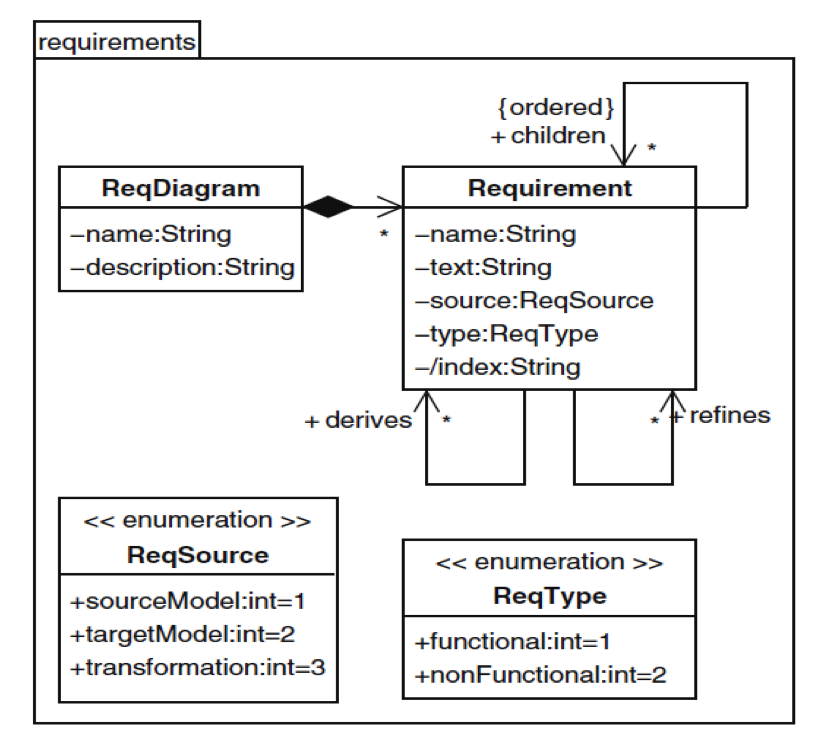
\includegraphics{transml-requirements.png}}}
\caption{\transml\ requirements metamodel}
\label{fig:transml-requirements}
\end{figure}

The requirements metamodel is very simple, but defines an expressive requirements language for BX. The language explicitly supports hierarchical decomposition of requirements, as well as classification, refinement, and traceability. Of particular note is the \textit{ReqSource} element, which identifies where a requirement arises, i.e., in the source of a transformation, the target of a transformation, or from the transformation itself (it is generated by the transformation). 

We illustrate the requirements metamodel with two examples, the first from Guerra et al \cite{GuerraLKPS13} which shows an example requirements model for a unidirectional transformation (Figure~\ref{fig:transml-requirements-example1}), and the second which shows an example for a BX (Figure~\ref{fig:transml-requirements-example2}). In both cases, the examples involve transformations from and between object-oriented and database models. We observe that different concrete syntaxes are used in each example. The first concrete syntax is based on SysML, whereas the second is a box-and-arrow domain-specific requirements language which makes use of elements of UML (particularly dependencies and stereotypes).

\begin{figure}[htbp]
\centering{\scalebox{0.6}{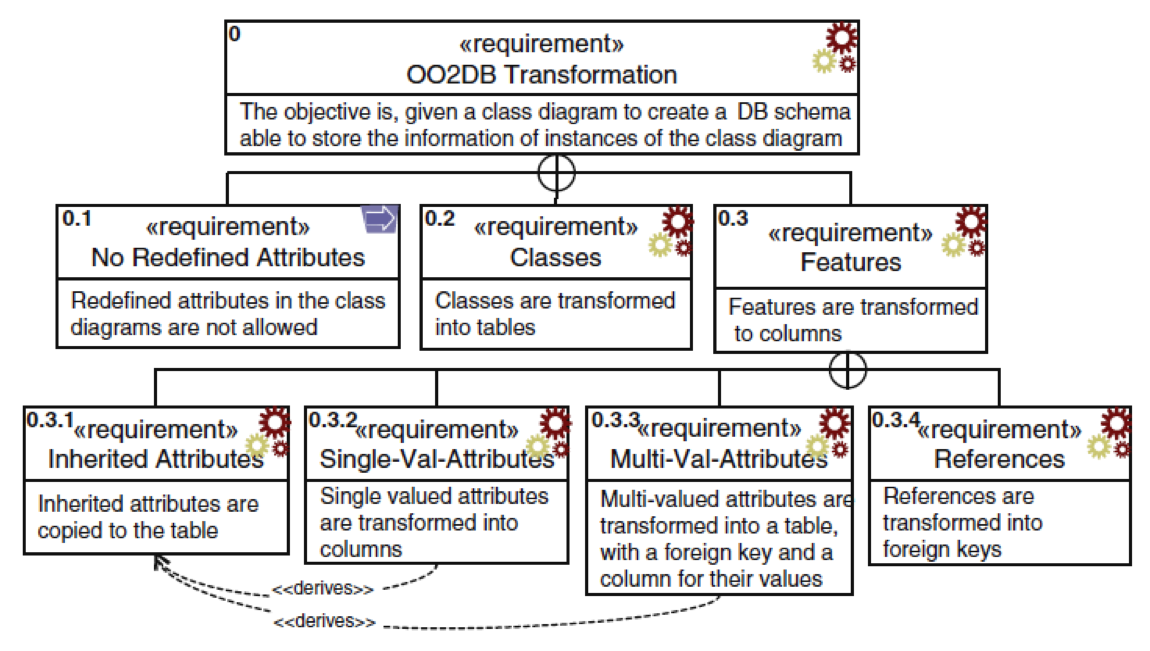
\includegraphics{transml-requirements-example1.png}}}
\caption{\transml\ requirements model example (SysML-like concrete syntax)}
\label{fig:transml-requirements-example1}
\end{figure}

The top-level requirement (OO2DB Transformation) in Figure~\ref{fig:transml-requirements-example1} is decomposed into the set of requirements below (i.e., No Redefined Attributes, Classes, Features). The Features requirement is further decomposed in the last level of the diagram. Note that derived requirements are also noted, i.e., that the Inherited Attributes requirement is derived from the Single-Val-Attributes and Multi-Val-Attributes requirements.

\begin{figure}[htbp]
\centering{\scalebox{0.6}{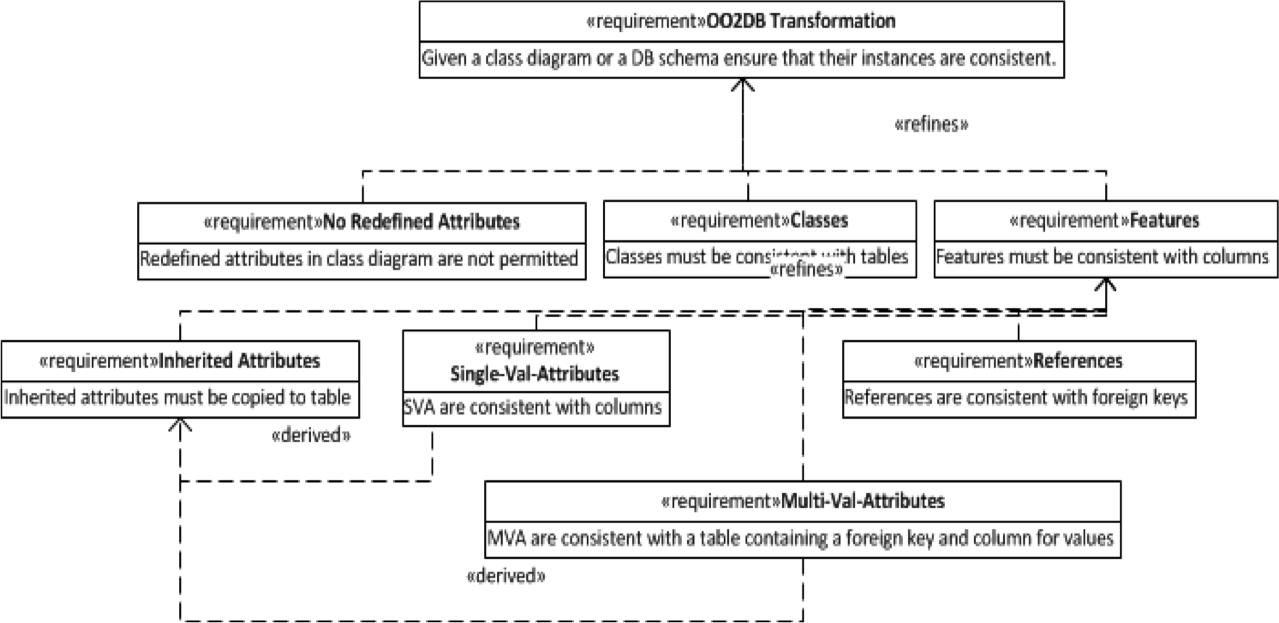
\includegraphics{transml-requirements-example2.png}}}
\caption{\transml\ requirements model example (box-and-arrow concrete syntax)}
\label{fig:transml-requirements-example2}
\end{figure}

The example in Figure~\ref{fig:transml-requirements-example2} illustrates a requirements specification for a BX. It has a similar structure to the previous example for a unidirectional transformation. The main difference is in the expression of the individual requirements, which are expressed in terms of consistency relationships rather than transformation features. 

Both of these examples are informal, in the sense that they rely substantial on natural language, and are the result of applying elicitation techniques; they may contain imprecision or inconsistencies, which may be resolved by analysis. \transml\ supports two sets of languages for requirements analysis: a simple scenario language, and a formal specification language for requirements. 

The simple scenario language of \transml\ supports description of \textit{concrete cases} for transformation, i.e., how examples are meant to be related by the BX. \transml\ is applicable to both models or fragments of models, the latter of which is essential for incremental development and for working with large monolithic models. An example of a transformation case (i.e., a scenario) for part of an object-oriented to database BX is shown in Figure~\ref{fig:transml-example-case}.

\begin{figure}[htbp]
\centering{\scalebox{0.6}{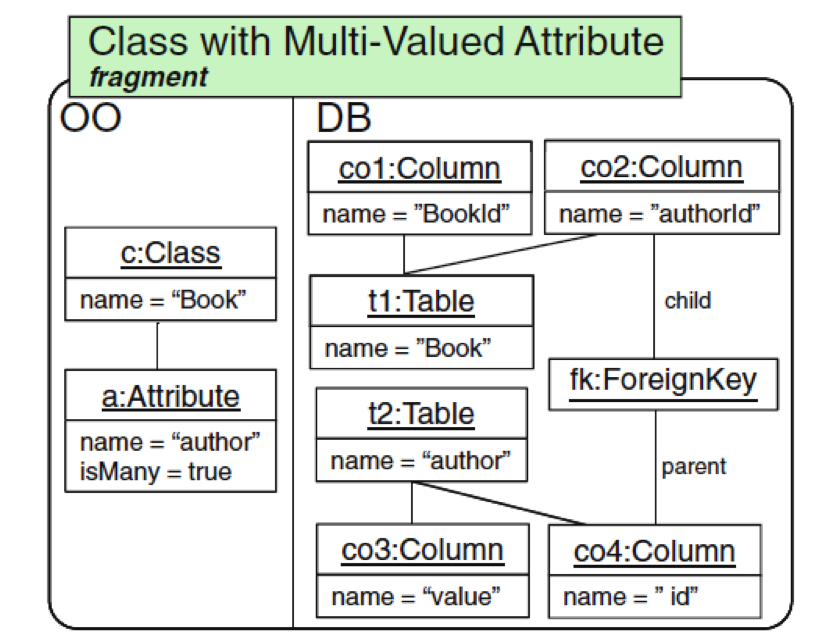
\includegraphics{transml-example-case.png}}}
\caption{\transml\ scenario (example case)}
\label{fig:transml-example-case}
\end{figure}

On the left side of the example is the object-oriented model fragment, consisting of a class with a multi-valued attribute; on the right side is a database model fragment, consisting of two tables containing columns and foreign keys. This is an example of a BX scenario involving a class with a multi-valued attribute and a consistent database model that resolves the multi-valued aspect using a foreign key (there are other solutions).

The second \transml\ language for requirements analysis supports formal specification of requirements; it is used to specify what a transformation has to do. It captures correctness properties and specifies restrictions on the models involved in the BX (for example, the consistency relations specified in the BX may only be applicable when the source or target models obey various constraints). \transml\'s formal specification language supports all of this via use of declarative patterns, a concept taken from triple graph grammars. Patterns express allowed and permitted relations between elements from the involved models. The pattern language itself is expressive and can include conditions on attribute values as well as constraint.

The metamodel for the \transml\ formal specification language for requirements is depicted in Figure~\ref{fig:transml-formal-language}.

\begin{figure}[htbp]
\centering{\scalebox{0.6}{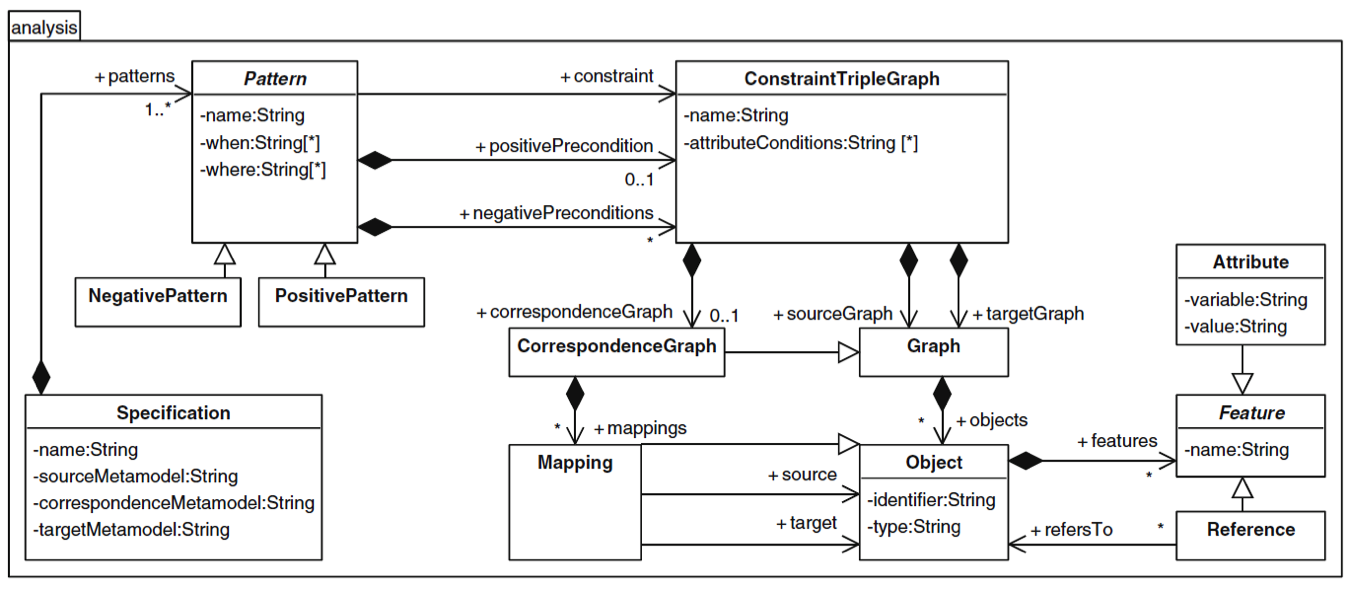
\includegraphics{transml-formal-language.png}}}
\caption{\transml\ formal specification language metamodel}
\label{fig:transml-formal-language}
\end{figure}

A requirements specification (the Specification element in Figure~\ref{fig:transml-formal-language} is made up of a number of patterns. A pattern may be a positive or a negative precondition, which are similar to both the \textit{when}-clauses of QVT Relations, as well as triple graph grammar's negative application conditions. The Constraint Triple Graph element encodes these clauses, and also include correspondence graphs (which is effectively traceability information) as well as links to source and target graphs. 

An example of a pattern for a BX is shown in Figure~\ref{fig:transml-pattern}. 

\begin{figure}[htbp]
\centering{\scalebox{0.6}{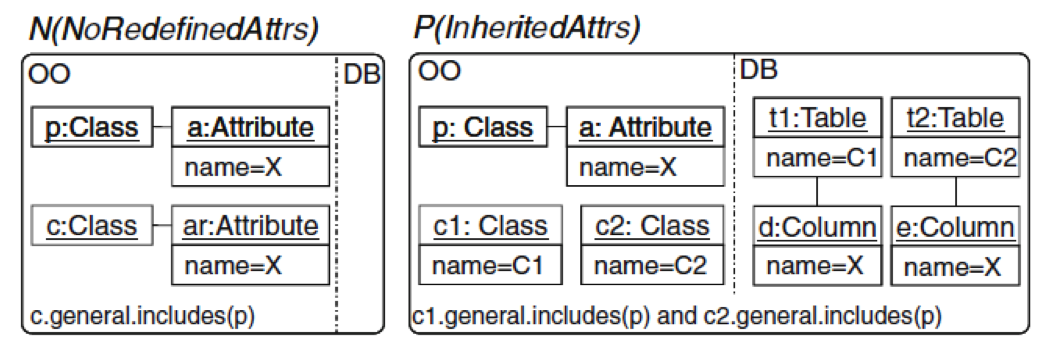
\includegraphics{transml-pattern.png}}}
\caption{\transml\ example pattern}
\label{fig:transml-pattern}
\end{figure}

The example pattern is, once again, taken from the object-oriented to database BX example that we have used several times before. In this example, the left side of the diagram is a negative pattern: it checks for the existence of two classes $c$ and $p$ such that $p$ is an ancestor or $c$, while both have an attribute with the same name ($X$). On the right is a positive pattern: it expresses the inherited attribute property (in this case, the inherited attribute named $X$ is mapped into two columns in the database model). More detailed examples of patterns and specifications can be found in \cite{GuerraLKPS13}.

In the next section we consider the next phases of the BX engineering lifecycle, focusing on architecture and design; we will explore further aspects of \transml\ for supporting these phases.



\section{Architecture and Design}
\label{section:architecture-and-design}

In this section we motivate and present an approach for developing the architecture and design of a BX, including MDE languages to capture detailed designs of BX, as well as techniques for expressing and applying design patterns for BX. What we present here builds on the techniques introduced in the last section, where we used \transml\ to capture requirements for BX.

As discussed earlier, large and complicated BX are similar to large and complicated software systems: they involve many parts (e.g., transformation components, rules) with complicated inter-relationships and dependencies. Many BX have sophisticated behaviour which can be difficult to interpret from their concrete syntax. They are also difficult to engineer correctly. Large software systems are usually not monolithic: they are built as a set of interrelated components. Arguably, BX should be constructed in the same way. 

Nevertheless, architecture for BX -- and transformations in general -- can be complicated. Some of the issues are as follows.
\begin{itemize}
\item \textit{Components:} what are appropriate component models for BX? For software systems we have a reasonable understanding of what a component in a software architecture is, how it may be implemented, and how it can be precisely combined with other components. Our understanding of components for BX and transformations in general is underdeveloped. Most transformation languages offer a notion of a \textit{rule}, and some languages have a notion of \textit{module}, but richer and deeper understanding (e.g., of ports, protocols, and architectural styles) is missing.

\item \textit{Relationships:} what are appropriate relationships that can be defined between BX components? For software systems we have a comprehensive library of component connectors (e.g., protocols, buffers, compositions, containments) that can be deployed; a similar understanding for BX is not yet available.

\item \textit{Interoperability:} a key aspect of software architecture is what it provides in terms of interoperation with external systems. For BX, the question is: how can a BX be integrated with other components or architectures, e.g., code generators, verification tools, etc. 
\end{itemize}

We will now present an approach to transformation architecture, embodied in \transml\, and present several small examples of both BX architecture and unidirectional transformation architecture. We then describe an approach for detailed design for transformations.

\subsection{BX Architecture in \transml\ }
In Section~\ref{section:requirements} we introduced the \transml\ approach and explained its support for requirements specification (including scenarios and formal requirement specification). As illustrated  in Figure~\ref{fig:transML}, \transml\ provides support for expressing transformation architectures and designs. 

Architecture in \transml\ is embodied in a traditional architectural modelling approach: an architecture is a set of components and connectors that interact via directional interfaces. Component types are given in terms of metamodels, or event types (for supporting event-driven architectures or for events generated by sensors) or other components (to support higher-order transformations). The component model is general in the sense that it can be used to represent transformations, black-box components (e.g., non-transformation or non-MDE components), or actors (e.g., human users). 

The \transml\ metamodel for architectures is illustrated in Figure~\ref{fig:transml-architecture}. It is worth noting the \textit{direction} attribute on the Interface element; components of BX may both generate and receive  information via interfaces.

\begin{figure}[htbp]
\centering{\scalebox{0.6}{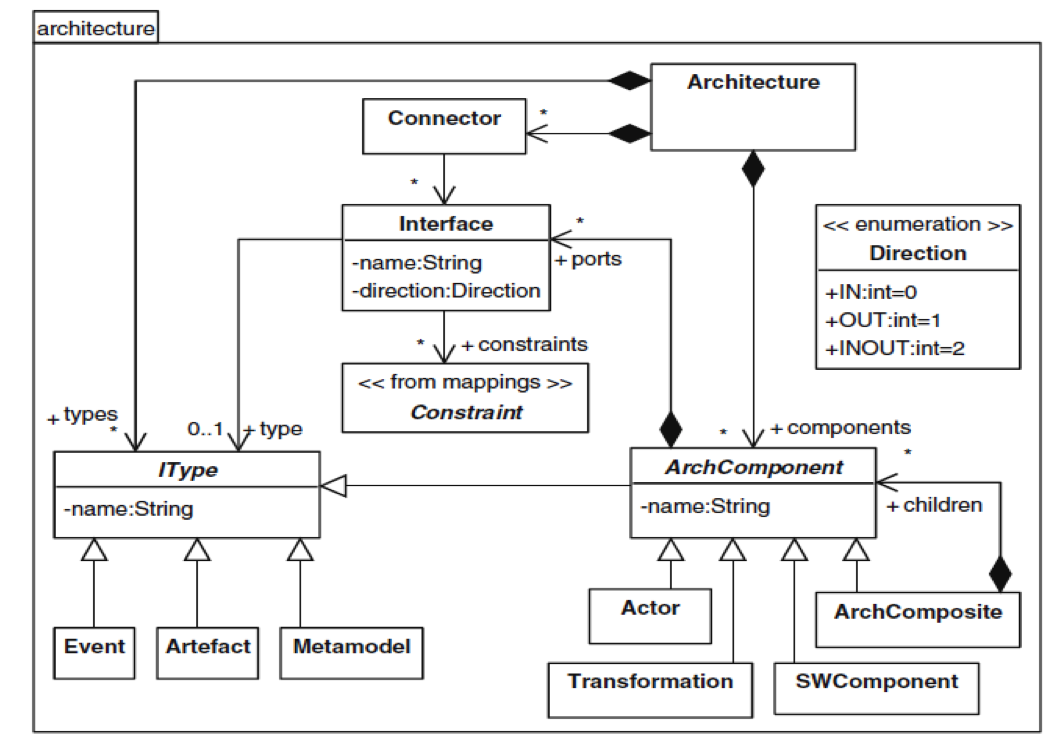
\includegraphics{transml-architecture.png}}}
\caption{\transml\ architecture metamodel}
\label{fig:transml-architecture}
\end{figure}

Constraints on interfaces can be used to impose a concept of contract, e.g., to restrict expected inputs and outputs, but also to support conformance checking.

Figure~\ref{fig:architecture-example1} shows an example of a unidirectional transformation architecture, using a simple component-based concrete syntax from UML. This example illustrates a transformation-centric view, i.e., the components in the architecture are themselves transformations. This can be contrasted with a type-centric architecture, shown in Figure~\ref{fig:architecture-example2}, where the components are types (or metamodels). In both cases, the example architecture is for a chain of transformations between an object-oriented model and SQL code.

\begin{figure}[htbp]
\centering{\scalebox{0.6}{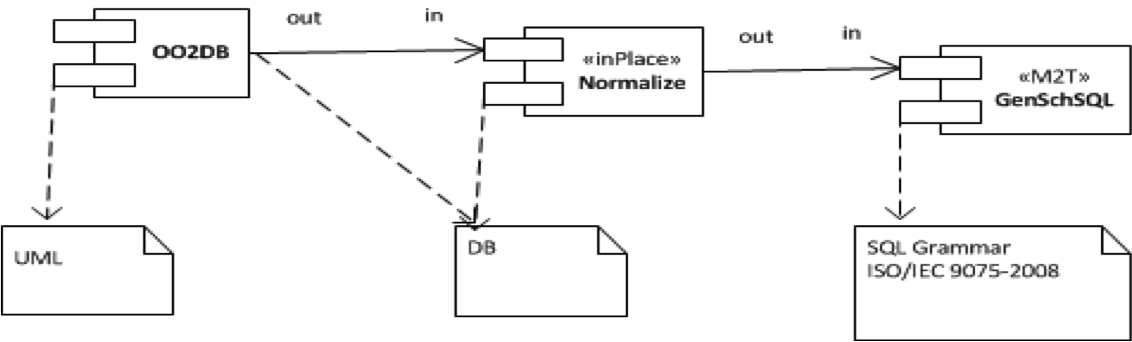
\includegraphics{transml-arch-example1.png}}}
\caption{\transml\ architecture example (transformation-centric)}
\label{fig:architecture-example1}
\end{figure}

In the above example, firstly a unidirectional OO2DB transformation is executed (taking a UML model as input and producing a DB model as output). Then, a normalising update-in-place transformation is executed on the DB model. Finally, a model-to-text transformation is executed on the DB model, producing SQL compliant to a specific grammar.

\begin{figure}[htbp]
\centering{\scalebox{0.6}{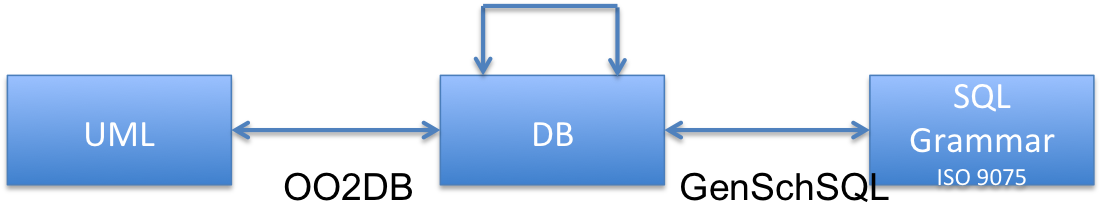
\includegraphics{transml-arch-example2.png}}}
\caption{\transml\ architecture example (type-centric, bidirectional)}
\label{fig:architecture-example2}
\end{figure}

The type-centric view represents the individual transformations as relationships between components. We have extended this example to represent bidirectional transformations throughout: i.e., the OO2DB, Normalise and GenSchSQL (the model-to-text transformation) could be executed in either direction.  We could, of course, present the same BX in a transformation-centric style. In this case, the architecture in Figure~\ref{fig:architecture-example1} would have bidirectional dependencies on the relevant input and output models, as depicted in Figure~\ref{fig:architecture-example3}.

\begin{figure}[htbp]
\centering{\scalebox{0.6}{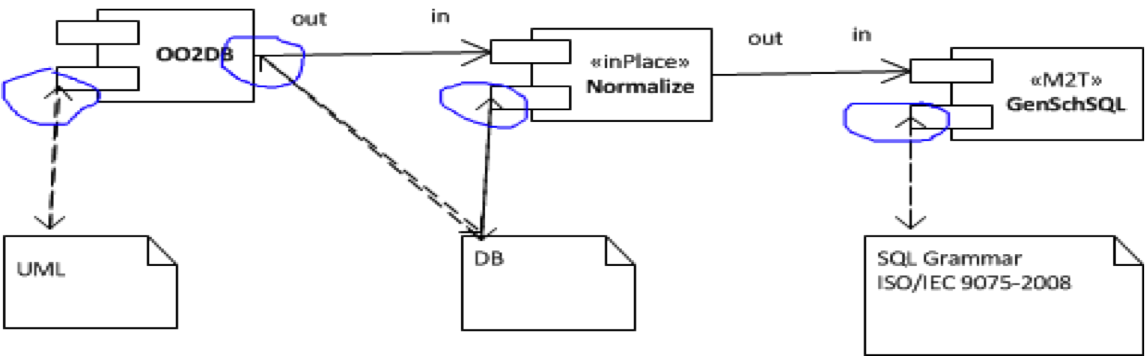
\includegraphics{transml-arch-example3.png}}}
\caption{\transml\ architecture example (transformation-centric, bidirectional)}
\label{fig:architecture-example3}
\end{figure}

\subsection{Design of BX}
The architecture of a software system captures the key components and their interrelationships. In the case of a BX this includes the connections between transformation components, the ports through which components communicate, and restrictions and constraints on that communication. The engineering process for BX continues with design, which can be broken into two parts: \textit{high-level design}, which focuses on capturing \textit{what is transformed into what}; and \textit{low-level design}, which focuses on capturing \textit{how} the transformation is to be carried out. We briefly consider \transml\ support for each aspect.

High-level design of a BX, once again, aims to capture what is transformed into what. To represent this, \transml\ introduces a \textit{mapping diagram}, inspired by triple graph grammars. These capture the mappings between arbitrary model elements involved in the transformation. However, mappings are not meant to be used as a implementation model -- specifically, they are not meant to be used as a tracing mechanism to guide the execution of code (this, as we will soon see, is the purpose of the low-level design features of \transml\).

The \transml\ metamodel for mapping diagrams is illustrated in Figure~\ref{fig:transml-mapping-diagram}. Mappings have ends which are associated with modelling elements. Navigability is a property of mappings; BX will involve navigation to both source and target. Constraints can be attached to mappings in order to define conditions on when (part of) a mapping can hold. 

\begin{figure}[htbp]
\centering{\scalebox{0.6}{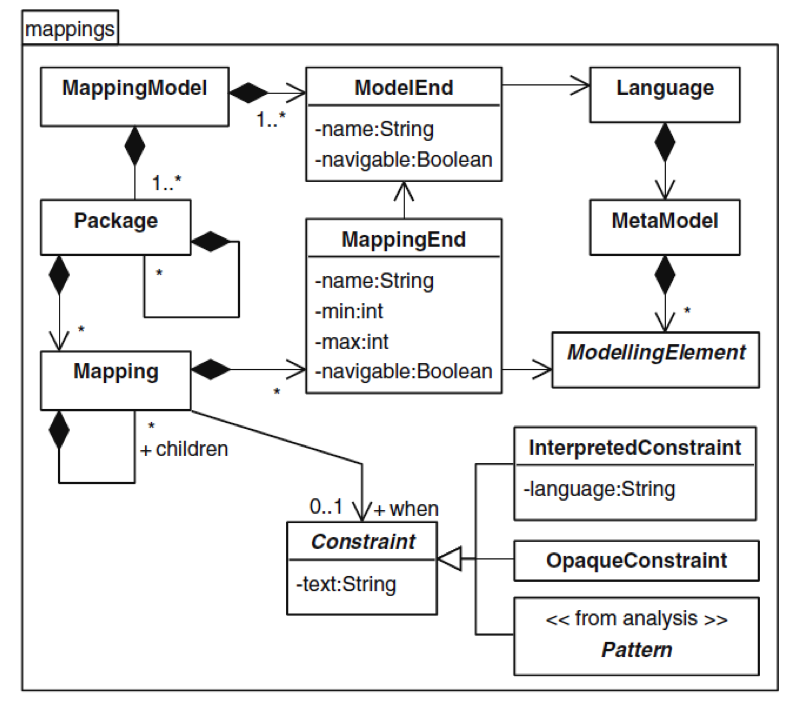
\includegraphics{transml-mapping-diagram.png}}}
\caption{\transml\ mapping diagram metamodel}
\label{fig:transml-mapping-diagram}
\end{figure}

Figure~\ref{fig:transml-mapping-example1} illustrates a mapping, for the Class2Relational BX. On the left of the diagram is a package containing key modelling elements of an OO model; on the right, a database model. In the centre are the mappings along with some informal English text explaining the purpose of each distinct mapping. Note the navigability of each rule; these can be executed from a DB model to an OO model, or vice versa.

\begin{figure}[htbp]
\centering{\scalebox{0.6}{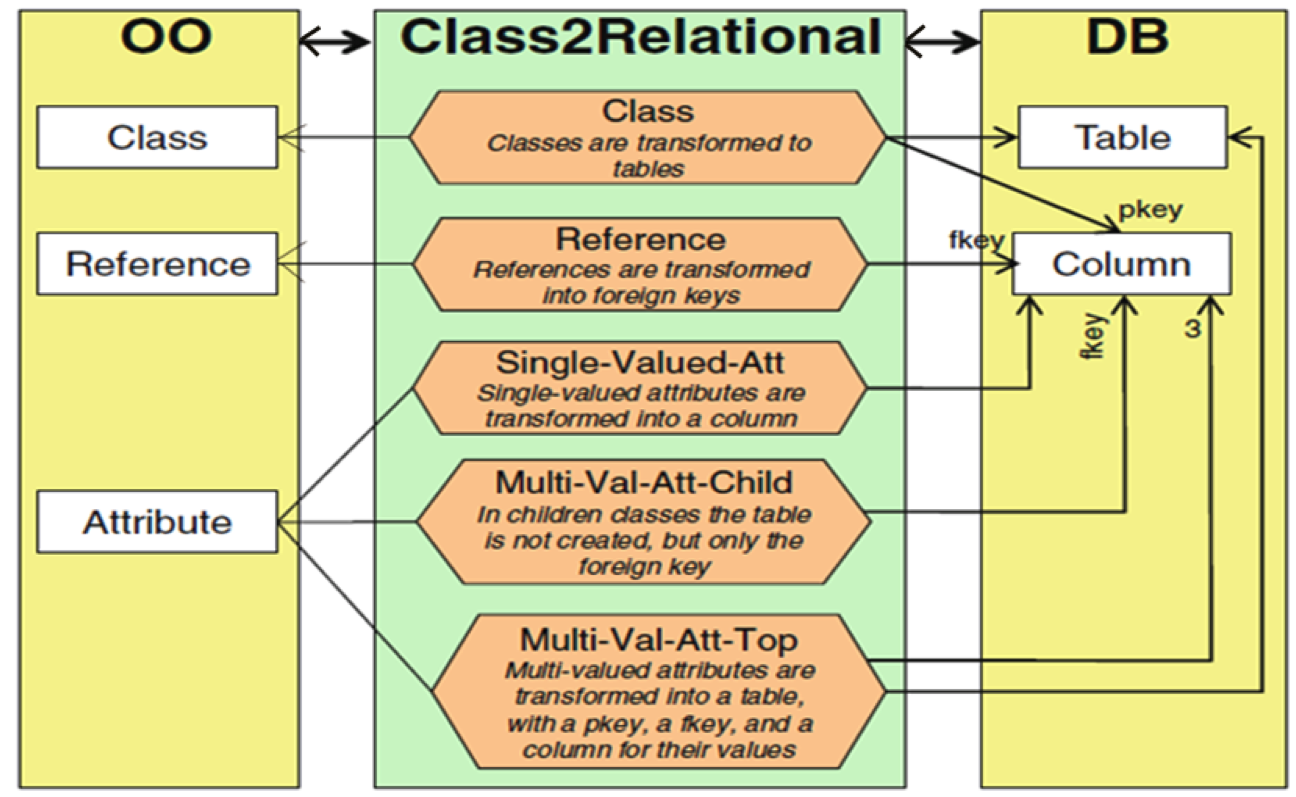
\includegraphics{transml-mapping-example1.png}}}
\caption{\transml\ mapping example}
\label{fig:transml-mapping-example1}
\end{figure}

The next example elaborates what is presented in Figure~\ref{fig:transml-mapping-example1} and imposes a constraint on the very last mapping, Multi-Val-Att-Top. The constraint, expressed in OCL, states that the owner of an attribute cannot have any parent classes; this is so that multi-valued attributes can be appropriately flattened into a table.

\begin{figure}[htbp]
\centering{\scalebox{0.6}{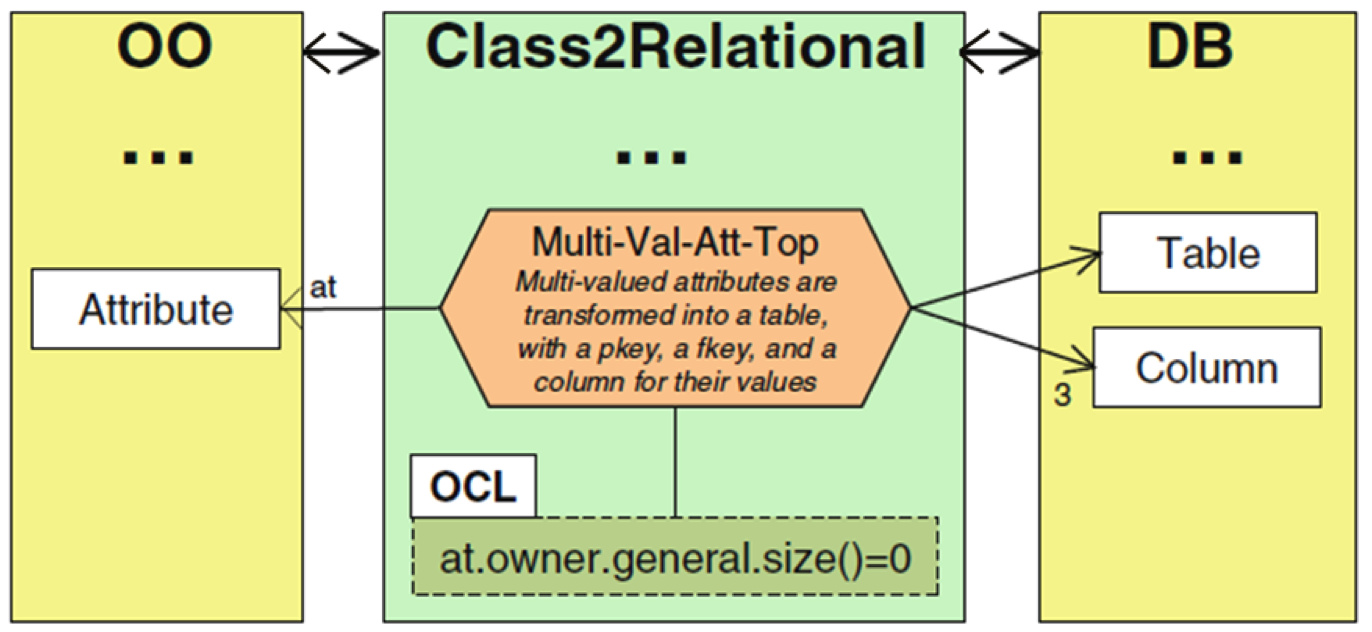
\includegraphics{transml-mapping-example2.png}}}
\caption{\transml\ mapping example (constraint)}
\label{fig:architecture-example3}
\end{figure}

While high-level design is supported in \transml\ via mapping diagrams, low-level design -- which is where the transition to implementation begins -- is
supported by more detailed diagrams. Technically, low-level design \textit{could} be supported by using a favourite BX programming language. But it may be preferable - for reasons of process - to maintain a degree of platform independence while still focusing on the essential aspects of BX development. As such, \transml\ provides low-level design languages for capturing the \textit{structure} of BX rules, control flow, and blocks. These are encapsulated in two diagrams: the \textit{rule structure diagram} and the \textit{rule behaviour diagram}.

The rule structure diagram (metamodel in Figure~\ref{fig:transml-rulestructure} is used to refine a mapping diagram. A rule can contribute to the implementation of one or more mappings. Rules themselves may be unidirectional or bidirectional. Structure diagrams also allow for explicit or implicit (e.g., nondeterministic) capture of execution flow, via subclasses of the \textit{Flow} metaclass. In particular, a set of rules can be placed inside a nondeterministic block, for example, as in graph transformation programs.




\section{Verification}
\label{section:verification}

\newcommand{\BX}{BX}

In this section we explore a specific approach to verifying BX. The approach we present is intended to be pragmatic, meant to be used with existing MDE tools and technologies. As such we do not consider issues such as soundness or completeness, though the mechanisms are present to prove conjectures related to these properties if so desired.

\BX\ are challenging to implement on account of the inherent complexity that they must encode. Model transformation languages supporting them often do so with conditions: some require that \BX\ are bijective (e.g.\ BOTL \cite{Braun-Marschall03a}), whereas others require users to work with specific formalisms such as triple graph grammars (e.g.\ MOFLON \cite{AKRS06a}).  Many modern transformation languages do not provide any support for \BX\ (e.g.\ ATL \cite{JABK08a}), meaning that users must express them as two unidirectional transformations. While this seems a practical workaround, the two transformations may diverge over time -- that is, there are no constructive guarantees that the two unidirectional transformations maintain the consistency relationship between the models being manipulated.
	
A trade-off between the benefits (but complexity) of pure \BX\ languages and the practicality (but possible incoherence) of unidirectional transformations can be achieved in Epsilon, a platform of interoperable and executable model management languages. Epsilon has languages supporting the specification of unidirectional transformations in either a rule-based (ETL), update-in-place (EWL), or operational (EOL) \cite{Paige-KRDP09a} style. Furthermore, it provides an inter-model consistency language (EVL \cite{Kolovos-Paige-Polack09a}) that can be used to express and evaluate constraints between models. With these languages, \BX\ can be ``faked'' by: (1) defining pairs of unidirectional transformations for separately updating the source and target models; and (2) defining inter-model constraints in EVL, the violation of which will trigger appropriate transformations to restore consistency.
	
Although this process gives us a means of checking consistency and automatically triggering a transformation to restore it, we lack the important guarantee that \BX\ give us: the compatibility of the transformations. It might be the case that after the execution of one transformation, the other does not actually restore consistency, leading to further EVL violations. Thus, how do we check for, and maintain, compatibility? 
	
We aim to obtain the guarantees of \BX\ without
the need for \BX\ languages. Instead, we can use \emph{rigorous} proof
techniques to verify that faked \BX\ are consistency preserving, and thus
indistinguishable to users from true \BX. To this end, we propose to apply
techniques from graph transformation verification. Given a faked \BX\ in
Epsilon, we will model the unidirectional transformations as graph
transformation rules, and EVL constraints as nested graph conditions
\cite{Habel-Pennemann09a}. Then, by leveraging graph transformation proof
calculi \cite{Habel-Pennemann-Rensink06a,Poskitt13a,Poskitt-Plump12a} in a
weakest precondition style, we aim to automatically prove compatibility of the
unidirectional transformations with respect to the EVL
constraints. 

\subsection{Illustration}
To illustrate the idea, consider yet again the OO to RDBMS problem. Class diagram models conform to a simple language describing familiar object-oriented concepts, whereas relational database models conform to a language describing how databases are constructed. Consistency is defined in terms of a correspondence between the data in the models, e.g.\ every table $n$ corresponds to a class $n$, and every column $m$ corresponds to an attribute $m$. Figure~\ref{fig:cd2rdbm_example} contains two simple models that are consistent in this sense (we omit the metamodels, but they are obvious).	

\begin{figure}[htbp]
\centering{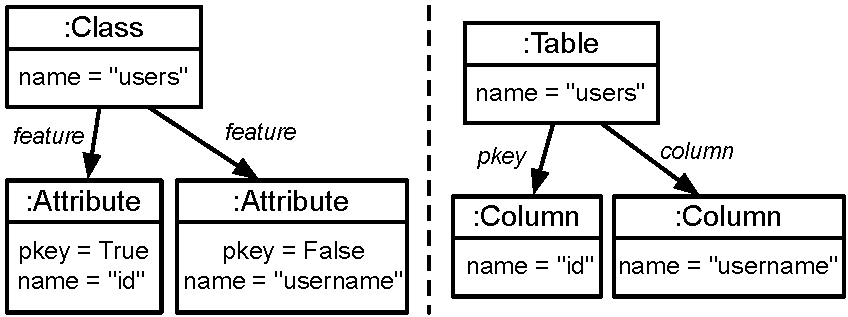
\includegraphics[width=0.6\textwidth]{cd2rdbm-ex.pdf}}
\caption{Two consistent OO and RDBMS models}
\label{fig:cd2rdbm_example}
\end{figure}

%	\begin{wrapfigure}[9]{r}{0.6\textwidth}
%		\centering
%			\vspace{-22pt}
%			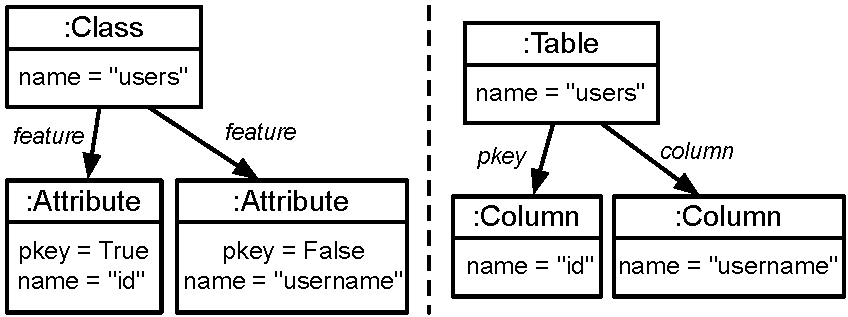
\includegraphics[width=0.6\textwidth]{cd2rdbm-ex.pdf}
%		\vspace{-21pt}\caption{Two consistent CD and RDB models}\label{fig:cd2rdbm_example}
%	\end{wrapfigure}
	
	Users of the models should be able to create new classes (or tables) whilst maintaining inter-model consistency. Upon the creation of a new class (resp.\ table), a table (resp.\ class) should be created with the same name to restore consistency. We can implement such a simple \BX\ in Epsilon with a pair of unidirectional transformations (one for updating the class diagram model, one for updating the relational database) and a set of EVL constraints. For the former, we can use the Epsilon Wizard Language (EWL) to define a pair of update-in-place transformations, $\tt AddClass$ and $\tt AddTable$ (for simplicity, here we assume the new class/table name $\tt newName$ to be pre-determined and unique, but Epsilon does support the capturing and sharing of such data between wizards).
	
%\vspace{-15pt}
%\begin{center}
%	\begin{minipage}[t]{0.475\textwidth}
	\begin{lstlisting}[language=java]
wizard AddClass {
 do {
   var c: new Class;
   c.name = newName;
   self.Class.all.first().contents.add(c);
 }}
 \end{lstlisting}
%	\end{minipage}
	\hspace{7pt}
%	\begin{minipage}[t]{0.475\textwidth}
	\begin{lstlisting}[language=java]
wizard AddTable {
 do {
   var table: new Table;
   table.name = newName;
   self.Table.all.first().contents.add(table);
 }}
	\end{lstlisting}
%	\end{minipage}
%\end{center}
%
%\vspace{-8pt}%

Using the Epsilon Validation Language (EVL), we express inter-model consistency: that for every class $n$, there exists a table named $n$ (and vice versa). If one of the constraints is violated, Epsilon can automatically trigger the relevant transformation to attempt to restore consistency. For example, after executing the transformation $\tt AddClass$, the constraint $\tt TableExists$ will be violated, indicating that the transformation $\tt AddTable$ should be executed to restore consistency.
	
%	\vspace{-15pt}\begin{center}
%		\begin{minipage}[t]{0.475\textwidth}
		\begin{lstlisting}[language=java]
context OO!Class {
 constraint TableExists {
   check : DB!Table.all.select(t|t.name = self.name).size() > 0
}}	
		 \end{lstlisting}
%		\end{minipage}
		\hspace{7pt}
%		\begin{minipage}[t]{0.475\textwidth}
		\begin{lstlisting}[language=java]
context DB!Table {
 constraint ClassExists {
   check : OO!Class.all.select(c|c.name = self.name).size() > 0
}}
		\end{lstlisting}
%		\end{minipage}
%	\end{center}	
%\vspace{-8pt}%

This example of a \BX, ``faked'' in Epsilon, is a simple one chosen to illustrate the concepts. Even what appears to be a simple \BX can lead to more interesting (i.e.\ less symmetric) \BX, e.g.\ manipulating inheritance in the class model.

\subsection{Checking Compatibility}
A critical difference between the ``faked'' \BX\ in the previous section and a true \BX\ is the absence of guarantees about the compatibility of the transformations: upon the violation of $\tt TableExists$, for example, does the execution of $\tt AddTable$ actually restore consistency? For this simple example, a manual inspection will quickly confirm that the transformations are indeed compatible. But what about more intricate \BX? And what about \BX\ that evolve and change over time? For the Epsilon-based approach to be a convincing alternative to a \BX\ language, it is imperative that the compatibility of the transformations can be checked, and that this can be done in a simple and automatic way. To this end, we propose to leverage and adapt some recent developments in the verification of graph transformations.
	
	Graph transformation is a computation abstraction: the state of a computation is represented as a graph, and the computational steps as applications of rules (i.e.\ akin to string rewriting in Chomsky grammars, but lifted to graphs). Modelling a problem using graph transformation brings an immediate benefit in visualisation, but also an important one in terms of semantics: the abstraction has a well-developed algebraic theory that can be used for formal reasoning. This has been exploited to facilitate the verification of graph transformation systems, i.e.\ calculi for systematically proving specifications about graph properties before and after any execution of some given rules. Furthermore, such calculi have been generalised to graph programs \cite{Plump12a}, which augment the abstraction with expressions over labels and familiar control constructs (e.g.\ sequential composition, branching) for restricting the application of rules. In particular, we look to exploit work by Poskitt and Plump who developed proof calculi for graph programs, separately addressing reasoning about programs and properties involving attribute manipulation \cite{Poskitt13a,Poskitt-Plump12a}, as well as reasoning about non-local structural properties \cite{Poskitt-Plump14a}.

Our example \BX\ for the OO2RDBMS problem is easily translated into graph programs and nested conditions, as given in Figure \ref{fig:ex-program-constraints}. The programs $P_S,P_T$ are the individual rules creating respectively a class or table node labelled $\tt newName$ (here, $\emptyset$ denotes the empty graph, indicating that the rules can be applied without first matching any structure, i.e.\ unconditionally). The nested condition $evl$, given on the right, expresses that for every class (resp.\ table) node, there is a table (resp.\ class) node with the same name (we do not define here a formal interpretation, but note that $\tt x,y$ are variables, and that the numbers indicate when nodes are the same down the nesting of the formula). Were the weakest liberal preconditions to be constructed, we would find:
	\[ \text{Wlp}(P_S;P_T,evl) \equiv \text{Wlp}(P_T;P_S,evl) \equiv evl. \]
	
	\noindent Since $evl \Rightarrow evl$ is clearly valid, both $\{evl\}\ P_S;\ P_T\ \{evl\}$ and $\{evl\}\ P_T;\ P_S\ \{evl\}$ must hold, and---assuming correctness of the abstractions---the original EWL transformations are therefore compatible with respect to the EVL constraints.
	
	\begin{figure}[htb]
\vspace*{-10pt}
		\centering
		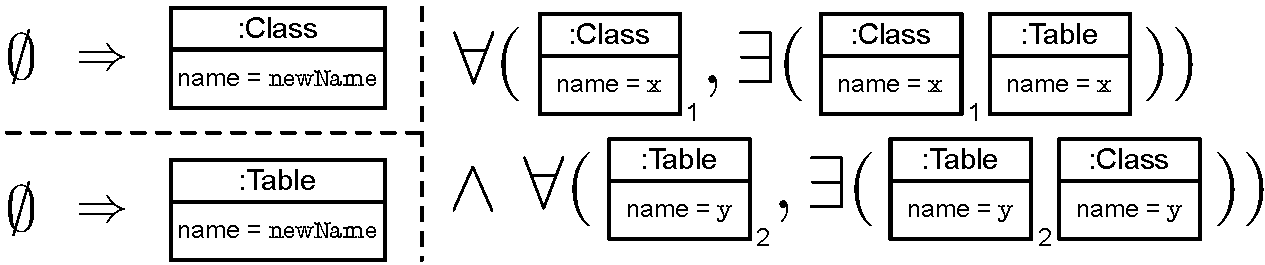
\includegraphics[width=0.8\textwidth]{ex-program-constraints.pdf}
		\caption{Our CD2RDBM \BX\ expressed as graph transformation rules and a nested condition}
\vspace*{-20pt}
		\label{fig:ex-program-constraints}
	\end{figure}

A key challenge with an approach such as this is what to do when the verification step fails, i.e., the implication above does not hold. We are exploring the use of the GROOVE tool to generate counterexamples when verification fails, via exploring executions of the graph transformation rules.


\section{Conclusions and Perspectives}
\label{section:conclusions}

Bidirectional transformations must be engineered, as must unidirectional transformations and other programs that manipulate models in MDE. The state-of-the-art in engineering BX is piecemeal at the moment: there are some specific techniques for supporting different engineering phases -- such as requirements engineering or design -- but very coarse understanding of efficient and effective engineering lifecycles, and alternative process models. This paper attempts to capture some of the current thinking on engineering BX. It summarises some of the state-of-the-art in BX design and implementation, presents some approaches for requirements specification and analysis, and suggests some ideas for capturing the architecture of complicated BX, and the detailed design of BX in general. It also presents some ideas on an approach for verification of BX; this approach is pragmatic, in the sense that it is meant to be used within an engineering process and it acknowledges tradeoffs between completeness and soundness.

MDE for BX possesses some sound theory -- such as delta lenses -- and some pragmatic, if incomplete, tools (such as Eclipse QVT-Relations) but these are still siloed: the theory needs to inform the enhancement of tools, and the tools need to be used to test the corners of the theory. A good example of research that attempts to link BX theory and practice is that combining triple graph grammars and delta lenses (e.g., \cite{0001EOCDXGE15}), but more needs to be done. What is really needed is tools that \textit{evidently} implement the theory in a systematic and audited way.

A key challenge in connecting theory with practical tools is the limitations in our theories of metamodelling. It is questionable whether we have a sound and complete understanding of a type theory for MDE and metamodelling, but this would underpin any attempts to link a theory of BX with the pragmatic tools supporting BX.

We mentioned tools for BX throughout this paper. The standardised tool in the MDE community is QVT-Relations; the Eclipse implementation is still under development. QVT-Relations has been criticised for being very complex, with substantial semantic ambiguity. The development of its Eclipse implementation is revealing some of these ambiguities, but this will only be convincing if supported by a sound theory, e.g., delta lenses. However, the gap between delta lens theory and QVT-Relations is substantial: changing QVT-Relations to conform with delta lenses may be difficult if not impossible; building a new BX that supports delta lens theory is possible, but it would not be QVT-Relations. It is difficult to see how connections between strong theory and MDE standards will play out. 

It also remains to be seen whether we can develop a rich, compelling set of industrial scenarios for BX. In our substantial industrial experience of transformations and MDE, we have had only one precise requirement for a BX (across over 20 industrial projects and 13 years of experience), and that was for the results of various forms of analysis (e.g., failure analysis, performance analysis) to be reflected on source models after calculation. It is unclear if such scenarios benefit from the heavyweight machinery of BX. But it should also be noted that requirements for BX sometimes emerge as development proceeds and having ways in which transformations can be \textit{extended} to become bidirectional may be useful.

In Section~\ref{section:verification} we described an approach to BX that involved specification of inter-model consistency constraints between two models, and the definition of two separate but synchronised update-in-place transformations on the two models. When the constraints were violated and the models became inconsistent, the transformations would be triggered to re-establish consistency. This approach -- two simple yet unidirectional transformations instead of a single bidirectional transformation -- needs to be clearly related to the BX solution space: when is it more effective to use versus building a full BX?

Finally, we observe that many transformations developed in practice are operational (e.g., those written in EOL or subsets of ATL). As well, there are many model-to-text (or model-to-grammar) transformations that support code generation scenarios. How do these fit in to the BX space? Are they simply too hard to consider? Are there scenarios or types of transformations that simple \textit{should not} (rather than \textit{cannot}) be bidirectionalised? As a challenge, consider the EuGENia tool\footnote{\url{https://eclipse.org/epsilon/doc/eugenia/}} which is a unidirectional model transformation written in EOL, which automatically generates three models needed by GMF to construct a graphical editor. These are generated by a transformation that takes as input a single annotated Ecore model. The transformation is defined entirely operationally, as we found that it would be too complex to implement using declarative rules (it is not a mapping transformation). Could EuGENia be turned into a bidirectional transformation? Our intuition is no (and, more pragmatically, we cannot see any reason why one would want to do so), but it would be interesting to explore what, fundamentally, makes an operational or hybrid transformation difficult to bidirectionalise.



\paragraph*{}\textbf{Acknowledgements} Parts of this work were supported by the European Commission's 7th Framework Programme, through grant \#611125 (MONDO).

\bibliographystyle{unsrt}
\bibliography{bibliography,references-amt}  % sigproc.bib is the name of the Bibliography 

\end{document}
